\chapter{智能复杂度迁移理论的形成与修正}
\label{chap:complexity-migration}

\begin{chapteroverviewbox}
本章讨论的是本书理论发展过程中一次重要但不能被简单删除的中间跃迁。在前面的讨论中，我们已经从 ``智能是多时空尺度上的多层嵌套闭环进程'' 出发，逐步建立了智能频谱、智能相、认知结构对象（CSO）以及 Agent-CSO 的区分。但是，在 CSO 本体最终形成以前，我们首先使用了一个更直观的概念来解释学习、熟练、记忆、工具使用和组织变化：\textbf{复杂度迁移（Complexity Migration）}。

复杂度迁移理论最初试图回答一个极其现实的问题：为什么一个新问题最初需要大量显式思考，而经过长期学习以后，却可以在几乎不进入工作记忆的情况下完成？如果任务本身并没有消失，那么原来占据工作记忆的 ``复杂度'' 去了哪里？由此我们曾提出：复杂度会在功能位置、时间尺度和系统边界之间迁移，并进一步尝试用复杂度密度、复杂度流和连续性方程描述这种变化。

然而，随着 CSO 与 Agent-CSO 理论的形成，我们逐渐认识到：\textbf{复杂度不是一种像能量一样能够独立流动的本体实体。真正发生迁移的是认知结构的表示形式、功能承载位置、时间尺度以及内部--外部载体。}因此，本章既保留复杂度迁移理论作为智能动力学的重要宏观描述，又对其本体论基础进行严格修正。

本章最终要完成如下理论转换：

\[
\boxed{
Complexity\ Migration
\quad\Longrightarrow\quad
Cognitive\ Structure\ Migration
}
\]

更准确地说，复杂度迁移应被理解为 CSO/Agent-CSO 承载变化在宏观统计层上的投影，而不是某种独立 ``复杂度物质'' 的运动。这个修正将成为下一章正式建立 CSO 迁移理论的前提。
\end{chapteroverviewbox}

\begin{figure}[htbp]
\centering
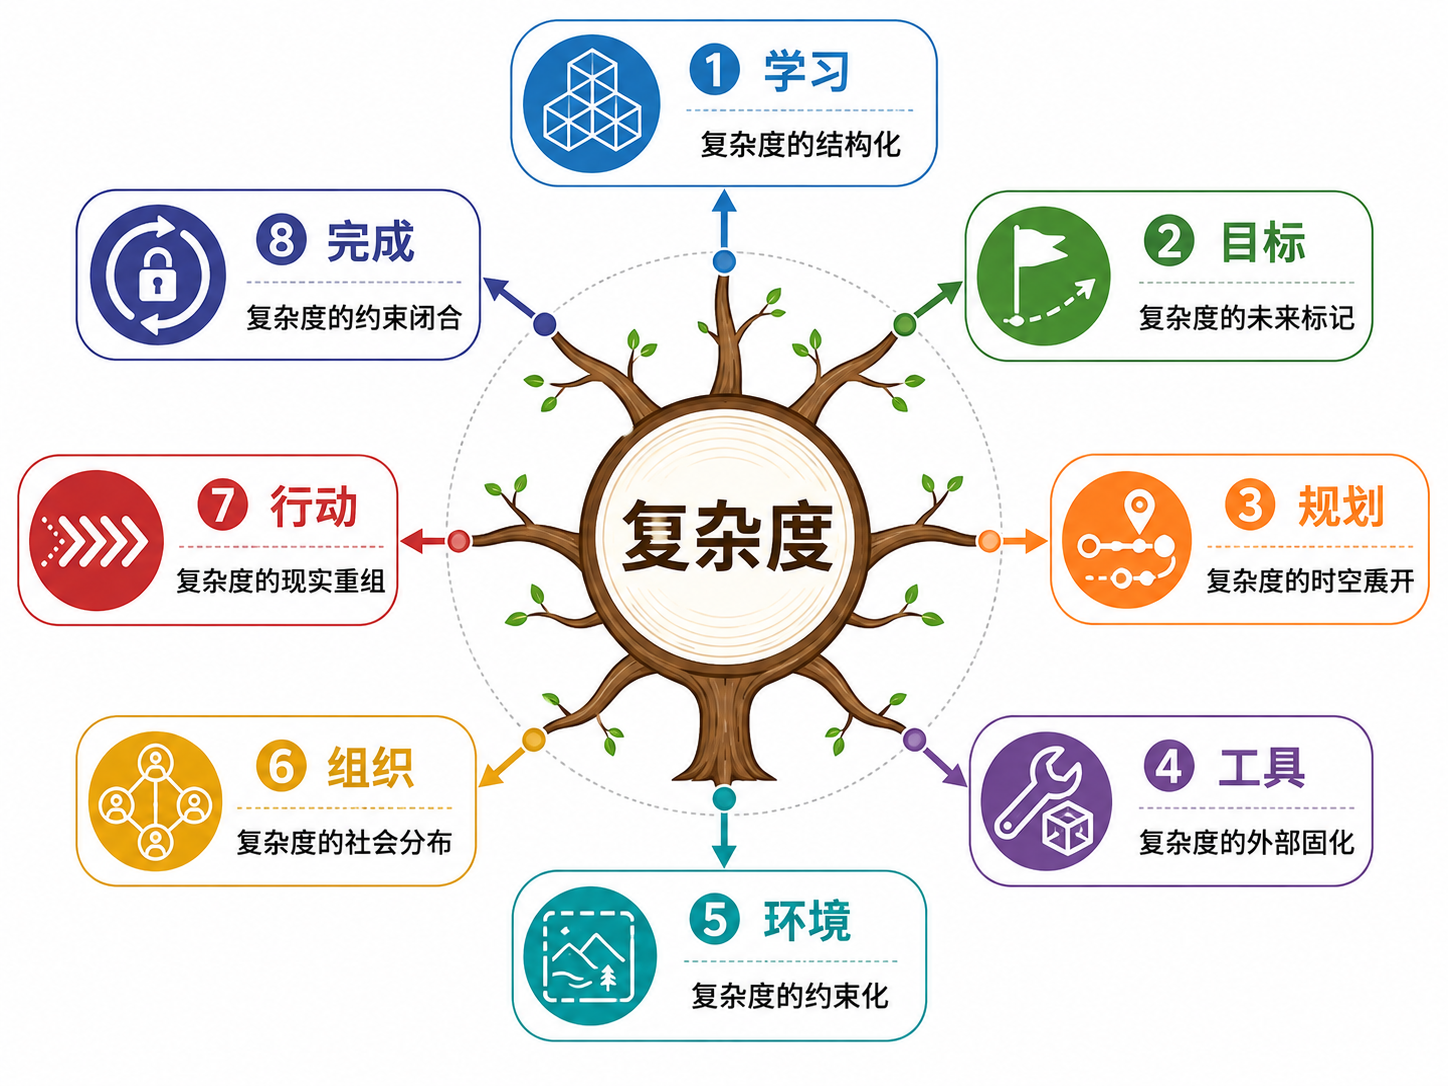
\includegraphics[width=.9\textwidth,height=.38\textheight,keepaspectratio]{images/complexity-migration-tree.png}
\caption{复杂度宏观描述及其结构来源}
\end{figure}

\section{为什么最初需要提出复杂度迁移}
\label{sec:why-complexity-migration}

我们首先回到这一理论最初产生的问题背景。一个初学者第一次解决某类问题时，往往需要在工作记忆中同时维持大量对象、规则、步骤、约束和中间状态。以一个从未使用过某类软件的 Agent 为例，它可能必须显式维护 ``当前窗口是什么''、``按钮在哪里''、``下一步操作会产生什么后果''、``任务目标是否已经满足'' 等大量关系。此时，任务对全局认知表面的占用是显著的。

但是，当同一个 Agent 重复执行数百次以后，情况通常发生变化。原来需要连续显式推理的过程开始变成稳定策略，甚至进一步变成程序、工具调用、低层控制器或者环境中的固定结构。此时，Agent 在完成同样外部任务时，其工作记忆中所需要显式维持的内容大幅下降。

这一现象给出了一个最初的理论直觉：

\[
\boxed{
Thinking\ Less
\neq
Task\ Disappearing
}
\]

如果任务仍然能够成功完成，而显式认知负担却下降，那么任务所需要的结构必然以某种方式被重新组织。早期理论因此把这种变化描述为：

\[
\boxed{
Complexity_{explicit}
\rightarrow
Complexity_{implicit}
}
\]

进一步，我们注意到这种变化并不仅发生在 ``显式--隐式'' 一个维度。熟练驾驶者对车辆姿态的控制可以从高层认知迁移到运动闭环；数学公式可以从一次次推导迁移到长期结构记忆；复杂计算可以迁移到计算器或程序；组织内部反复发生的人际协调可以沉降成岗位、流程和制度。换言之，原本必须由某一功能层承担的处理负担，后来可能由另一个功能层、另一个时间尺度乃至另一个外部载体承担。

于是，早期理论逐渐形成如下基本命题：

\[
\boxed{
Learning
\approx
Redistribution\ of\ Effective\ Complexity
}
\]

这里所谓 ``有效复杂度''，并不是任务在宇宙中的全部物理复杂度，而是相对于某一个智能体、某一个观察尺度和某一个当前功能位置而言，系统为了维持任务可解性而必须承担的结构负担。一个复杂任务本身可能没有变简单，但如果大量关系已经被压缩成一个稳定技能，那么对于工作记忆而言，它所表现出的运行复杂度就已经显著降低。

这也是为什么复杂度迁移理论最初具有很强的工程解释力。它把记忆、熟练、工具、环境改造和社会分工统一成同一种宏观现象：\textbf{复杂度并不总是被 ``消灭''，而是改变了由谁承担、在哪里承担以及以什么速度承担。}

如果用一个最简单的分解表示，我们曾把一个任务在当前 Agent 中产生的有效负担写成：

\[
C_{\mathrm{eff}}(t)
=
C_{\mathrm{run}}(t)
+
C_{\mathrm{stored}}(t)
+
C_{\mathrm{external}}(t)
+
C_{\mathrm{struct}}(t)
\]

其中 $C_{\mathrm{run}}$ 表示当前运行态显式处理负担，$C_{\mathrm{stored}}$ 表示已经进入记忆而不需要持续激活的结构，$C_{\mathrm{external}}$ 表示已经由工具、环境或其他主体承担的部分，而 $C_{\mathrm{struct}}$ 表示已经沉降进稳定技能、程序或功能连接中的结构。

这个公式从一开始就不应被理解为严格物理守恒关系。它真正表达的是一个认知工程直觉：\textbf{系统性能的提高常常不是因为所有问题结构都消失了，而是因为需要被中央显式处理的那一部分越来越少。}

因此，复杂度迁移理论最早并不是为了建立一个抽象形而上学，而是为了回答 AgentOS 中一个最现实的问题：

\begin{statementbox}
如何让有限工作记忆只承担当前真正需要全局处理的结构？
\end{statementbox}

这一问题后来直接通向工作记忆有限容量定理、CCM、Offloading、Boundary、Body Skill 以及整个多尺度 AgentOS 架构。

\section{复杂度不是信息量：有效认知复杂度的定义}
\label{sec:effective-cognitive-complexity}

复杂度迁移理论要成立，首先必须解决一个定义问题：什么是我们所说的 ``复杂度''？如果把复杂度简单等同于数据量、token 数、参数数量或者 Shannon 信息熵，那么大量实际认知现象无法得到解释。

例如，一段包含一万个随机字符的字符串可能具有很高的信息熵，却未必对一个 Agent 构成高认知复杂度，因为 Agent 可以直接忽略它。相反，一个只有几十个符号的逻辑约束系统，如果内部关系高度耦合，却可能对工作记忆造成巨大压力。因此，AgentOS 讨论的复杂度首先是一种\textbf{结构相关、主体相关并且运行状态相关的有效认知复杂度}。

可以首先定义一个认知状态中的活动结构集合：

\[
\mathcal{X}(t)
=
\left\{
x_1(t),x_2(t),\ldots,x_n(t)
\right\}
\]

其中每一个 $x_i$ 可以代表当前需要维持的目标、关系、假设、约束、记忆片段、动作方案或中间变量。假设每个结构项具有局部负担：

\[
c_i(t)
\]

并具有当前激活权重：

\[
w_i(t)\in[0,1]
\]

则最简单的运行复杂度可写成：

\[
C_{\mathrm{run}}(t)
=
\sum_i w_i(t)c_i(t)
\]

但是，仅有加权和仍然无法描述结构之间的相互依赖。真正困难的推理往往不是因为对象多，而是因为关系密。为此，可以进一步引入活动结构图：

\[
\mathcal{G}_h(t)
=
\left(
V_h(t),E_h(t)
\right)
\]

其中 $V_h$ 表示当前进入工作记忆的结构节点，而 $E_h$ 表示必须同时保持的关系。于是有效认知复杂度可以概念性写成：

\[
C_{\mathrm{eff}}(t)
=
\alpha |V_h(t)|
+
\beta |E_h(t)|
+
\gamma \Phi(\mathcal{G}_h(t))
+
\delta U(t)
\]

其中 $\Phi$ 用于描述图的耦合强度、环结构、路径依赖或者非局部约束，而 $U(t)$ 表示不确定性、冲突和状态漂移带来的额外负担。

这个定义非常关键，因为它意味着：同样数量的信息，如果经过结构压缩，可以表现出完全不同的认知复杂度。假设十个彼此独立的规则经过学习后被压缩成一个更高层模式 $z$，那么：

\[
\{r_1,\ldots,r_{10}\}
\rightarrow
z
\]

虽然底层知识并没有消失，但工作记忆只需要激活 $z$，于是：

\[
C_{\mathrm{run}}^{\mathrm{after}}
<
C_{\mathrm{run}}^{\mathrm{before}}
\]

这正是抽象、概念化和技能化的核心认知收益之一。

在这个意义上，复杂度迁移理论从一开始就与压缩理论具有关系，但不能直接等同于压缩。压缩只是降低显式表示尺寸的一种方式，而迁移还可能把某种结构移动到另一个时间尺度或功能载体。例如，一个稳定技能即使内部控制器依然非常复杂，对于高层 Agent 而言，也可以通过一个极低维的控制接口表现：

\[
u_{\mathrm{high}}
=
\texttt{execute(skill)}
\]

内部则执行：

\[
x_{t+1}
=
F_{\mathrm{skill}}(x_t,u_t)
\]

因此，高层复杂度降低不意味着底层系统变简单，而意味着复杂度被封装进了稳定闭环。

由此，我们可以得到一个重要的相对性原则：

\[
\boxed{
Complexity
=
Complexity(
Structure,
Observer,
Carrier,
Timescale
)
}
\]

也就是说，复杂度并不是一个对象脱离主体和尺度以后仍然保持不变的绝对属性。同一结构对不同 Agent、不同功能层甚至同一 Agent 的不同发展阶段，都可能表现出不同有效复杂度。

这也解释了为什么后来的 CSO 理论必须出现。因为一旦复杂度本身取决于承载方式，我们就必须进一步追问：\textbf{究竟是什么结构在改变承载方式？}复杂度只能告诉我们 ``当前负担多大''，却不能充分告诉我们 ``什么东西正在被重新组织''。这个问题最终将导致本章后半部分从 Complexity 向 CSO 的本体转移。

\section{复杂度的功能迁移}
\label{sec:functional-complexity-migration}

复杂度迁移理论最早得到清晰形式化的方向，是\textbf{功能迁移（functional migration）}。所谓功能迁移，是指同一个任务相关结构不再由原来的认知功能承担，而逐渐被另一个功能层接管。

设一个智能系统具有功能集合：

\[
\mathcal{F}
=
\{F_1,F_2,\ldots,F_m\}
\]

在某一时刻，一个任务结构 $X$ 主要由功能 $F_i$ 承担：

\[
X@F_i
\]

随着经验增加，系统可能找到更稳定、更低成本的处理方式，使同样任务逐渐由 $F_j$ 承担：

\[
\boxed{
X@F_i
\rightarrow
X@F_j
}
\]

这就是最初意义上的功能复杂度迁移。

最典型的例子是从显式推理向程序化技能的迁移。一个机器人第一次抓取特殊物体时，可能需要高层规划器显式计算姿态、碰撞、接触位置和运动轨迹。但经过大量重复后，这些关系可以被局部预测控制器吸收。此时，高层系统只发出：

\[
Goal_{\mathrm{grasp}}
\]

而底层闭环自主解决：

\[
Perception
\rightarrow
Prediction
\rightarrow
Control
\rightarrow
Residual
\rightarrow
Correction
\]

从高层视角看，原本必须在工作记忆中维持的结构已经 ``消失''；实际上，它并没有消失，而是被封装进更低层、更快速、更稳定的功能闭环。

因此，我们曾提出：

\[
\boxed{
StableComplexity
\rightarrow
LowerLevelCarrier
}
\]

这一规律后来被重新表述成：

\[
\boxed{
StableCSO
\rightarrow
StableLocalFunctionalCarrier
}
\]

同样的结构也存在于纯数字 Agent 中。第一次完成一项复杂文件转换任务时，Agent 可能需要显式规划几十个步骤；若该过程不断重复，最终可生成一个脚本：

\[
\pi_{\mathrm{explicit}}
\rightarrow
Program
\]

以后工作记忆不再承担原有步骤链，只需要知道：

\[
\texttt{call(program)}
\]

这里发生的正是功能责任迁移。

这种现象让我们认识到，成熟智能的一个关键标志并不是 ``显式思考越来越多''，而恰恰可能是：

\[
\boxed{
\frac{
ExplicitGlobalProcessing
}{
SuccessfulBehavior
}
\downarrow
}
\]

随着能力成熟，越来越多稳定结构被迁移到局部功能闭环、高效程序、结构记忆或者外部工具，因此全局认知只处理异常、新颖和需要跨域协调的问题。

这也进一步形成了后来的重要原则：

\begin{statementbox}
NormalDynamicsStayLocal
\end{statementbox}

以及：

\begin{statementbox}
UnexpectedResidualEscalatesGlobally
\end{statementbox}

即正常、熟悉、低残差的过程应该尽量在局部完成，而只有局部无法解释或无法控制的残差才向上升级进入更昂贵的全局认知。

从这里可以看到，复杂度功能迁移并不是一个孤立概念。它后来直接演化成为 AgentOS 的层级控制原则、技能编译原则、BPCC 局部闭环原则以及 CSO 功能迁移理论。

\section{复杂度的时间尺度迁移}
\label{sec:timescale-complexity-migration}

功能位置之外，第二个重要维度是\textbf{时间尺度迁移}。智能系统中的结构并不是以同样速度变化。工作记忆可以在秒级变化，情景记忆在分钟到天的时间尺度逐渐积累，而结构记忆、自我以及生命周期生成先验则可能以更慢速度演化。

因此，我们早期提出：认知复杂度不仅存在于某一个位置，还存在于某一个特征频率或时间尺度上。

设某个认知结构具有特征时间尺度：

\[
\tau
\]

或者等价频率：

\[
\omega
\sim
\tau^{-1}
\]

那么学习可以表现成结构活动从高频向低频迁移：

\[
\boxed{
\omega_{\mathrm{fast}}
\rightarrow
\omega_{\mathrm{slow}}
}
\]

其认知意义是：原本需要持续、快速、显式更新的结构逐渐稳定下来，成为变化较慢的经验或生成结构。

这与三相记忆之间存在天然对应关系：

\[
h
\rightarrow
E
\rightarrow
\Theta
\]

可以被理解成：

\[
FastActiveStructure
\rightarrow
MediumTrajectoryStructure
\rightarrow
SlowGenerativeStructure
\]

第一次遭遇一个新现象时，大量相关关系停留在 $h$ 中；经过多次经历，这些关系形成 $E$ 中的经验轨迹；再经过抽象和整合，最终成为 $\Theta$ 中较慢的结构。

因此，我们可以把 ``巩固'' 写成：

\[
\boxed{
Fast
\rightarrow
Slow
}
\]

但这并不是单向过程。慢结构也会重新激活成快速活动：

\[
\boxed{
Slow
\rightarrow
Fast
}
\]

例如一个已经稳定存在于 $\Theta$ 中的数学规则，在当前问题中被召回以后重新进入 $h$，成为实时推理的一部分。

因此，认知结构的时间尺度迁移实际上是双向的：

\[
\boxed{
Consolidation:
Fast\rightarrow Slow
}
\]

\[
\boxed{
Activation:
Slow\rightarrow Fast
}
\]

这一点非常重要，因为它避免了把学习理解成单纯 ``越来越慢''。成熟智能必须同时具备把经验沉降成慢结构和在需要时快速重新激活这些结构的能力。

我们后来进一步尝试定义一个频谱上的复杂度密度：

\[
\rho_C(\omega,t)
\]

表示在时间 $t$，系统需要在特征频率 $\omega$ 附近承担多少有效结构负担。若加入功能位置 $f$，则有：

\[
\rho_C(f,\omega,t)
\]

从而可以把智能状态看成分布在：

\[
FunctionalSpace
\times
FrequencySpace
\]

上的结构分布。

这便是后来 ``智能频谱迁移'' 思想的来源。

但是，我们必须在这里提前指出一个后来的修正：$\rho_C$ 并不是像物理系统中的质量密度那样对应一种独立实体。它更接近一个\textbf{统计观测量}，描述多少 Agent-CSO 在什么功能和时间尺度上处于活动、稳定或承载状态。下一章会将其正式改写为：

\[
\rho_{CSO}(f,\omega,t)
\]

也就是说，真正有本体意义的是结构，而复杂度只是结构分布的一种宏观函数。

\section{复杂度的边界迁移与认知卸载}
\label{sec:boundary-complexity-migration}

第三种复杂度迁移发生在系统边界上。智能体并不需要把所有需要使用的结构永久保存在内部。相反，成熟智能往往具有极强的外化能力。

一个简单例子是电话号码。若一个人必须完全依靠生物记忆保存所有联系人号码，则这些信息必须占据内部记忆资源；当号码被写入手机以后，内部只需要保留：

\[
\text{``联系人可以在手机中找到''}
\]

于是原来的高维信息被迁移到外部载体。

对于 AgentOS，这一过程更加一般。可以定义内部结构集合：

\[
\mathcal{M}_{\mathrm{int}}
\]

以及外部可调用结构集合：

\[
\mathcal{M}_{\mathrm{ext}}
\]

则某个任务相关结构可能发生：

\[
X:
\mathcal{M}_{\mathrm{int}}
\rightarrow
\mathcal{M}_{\mathrm{ext}}
\]

外部载体可以是：

\[
File,\quad
Database,\quad
Script,\quad
Program,\quad
Tool,\quad
Environment,\quad
OtherAgent
\]

因此，我们曾经把这种现象描述为：

\begin{statementbox}
ComplexityOffloading
\end{statementbox}

也就是认知复杂度卸载。

但从更严格角度看，卸载并不是简单把负担 ``丢出去''。如果 Agent 完全忘记外部结构在哪里以及如何使用，那么这不构成有效的认知卸载，而只是信息丢失。真正的卸载要求内部保留某种\textbf{索引结构}：

\[
I_X
=
(
Location,
AccessMethod,
Validity,
Cost,
Trust
)
\]

于是完整过程更像：

\[
X_{\mathrm{internal}}
\rightarrow
I_X^{\mathrm{internal}}
+
X_{\mathrm{external}}
\]

内部保留一个低维导航结构，复杂内容则由外部载体承担。

这解释了为什么 ``外部记忆'' 并不是任何外界对象，而必须是 Agent 已经建立稳定访问关系的外部结构。

认知卸载理论后来又进一步扩展到环境改造。例如，一条经常需要绕行的路线，如果通过建造道路被永久改变，那么 Agent 并不是简单记住了一个新策略，而是直接修改了未来任务结构：

\[
Environment
\rightarrow
Environment'
\]

使得未来问题本身变得更容易。

因此：

\[
\boxed{
ChangeEnvironment
=
ChangeFutureCognitiveProblem
}
\]

这使环境成为一种极其特殊的外部认知载体。

类似地，在社会环境中，一个 Agent 还可以把任务委派给另一个 Agent，使：

\[
X@Agent_A
\rightarrow
X@Agent_B
\]

从个体视角看，这同样是边界迁移。

这也解释了社会分工的认知意义：文明并不是要求每个人掌握全部结构，而是通过制度、职业、工具和信息系统，把巨大的问题空间分布到不同载体中。

从早期复杂度语言看：

\[
\boxed{
C_{\mathrm{internal}}
\rightarrow
C_{\mathrm{external}}
}
\]

从后来的 CSO 语言看，则更精确地变成：

\[
\boxed{
AgentCSO:
B_{\mathrm{internal}}
\rightarrow
B_{\mathrm{external}}
}
\]

这里真正变化的是结构承载边界，而不是一种抽象复杂度物质。

\section{复杂度频谱与迁移流}
\label{sec:complexity-spectrum-flow}

在功能迁移、时间尺度迁移和边界迁移逐渐清晰以后，我们曾经尝试建立一个统一数学框架，将智能系统理解为 ``复杂度在功能--频率空间中的分布与流动''。

设：

\[
f\in\mathcal F
\]

表示功能位置，而：

\[
\omega\in\Omega
\]

表示时间频率，则定义复杂度密度：

\[
\rho_C(f,\omega,t)
\]

直觉上，$\rho_C(f,\omega,t)$ 表示在时刻 $t$，系统在功能位置 $f$ 和时间尺度 $\omega$ 上承载的有效认知复杂度。

进一步引入复杂度流：

\[
\mathbf J_C(f,\omega,t)
\]

其方向可以同时包含功能迁移方向与频率迁移方向：

\[
\mathbf J_C
=
\left(
J_F,
J_\omega
\right)
\]

如果再加入边界维度 $b$，则完整空间可以写成：

\[
\mathcal X_C
=
\mathcal F
\times
\Omega
\times
\mathcal B
\]

复杂度密度：

\[
\rho_C(f,\omega,b,t)
\]

复杂度迁移流：

\[
\mathbf J_C
=
(
J_F,
J_\omega,
J_B
)
\]

在最初理论中，我们进一步借鉴连续介质中的连续性方程，写出：

\[
\frac{\partial \rho_C}{\partial t}
+
\nabla\cdot\mathbf J_C
=
S_C-D_C
\]

其中：

\[
S_C
\]

表示新的复杂结构被引入系统，例如新问题、新环境、新知识；而：

\[
D_C
\]

则表示结构被删除、遗忘、合并、压缩或者变得不再相关。

这个形式的价值并不在于声称 ``复杂度真的像流体一样流动''，而在于它第一次把许多原本分离的 Agent 现象放进统一坐标中。

例如：

\[
J_\omega<0
\]

可以表示从快频向慢频的稳定化；

\[
J_\omega>0
\]

可以表示慢结构被重新激活；

\[
J_F
\]

可以表示不同功能之间的处理责任迁移；

\[
J_B
\]

可以表示内部向外部或者外部向内部的载体迁移。

于是：

\[
MemoryConsolidation,
SkillLearning,
Recall,
Offloading,
ToolUse
\]

在形式上都成为同一个迁移框架下的不同方向。

然而，这个模型也暴露了早期理论的核心问题：如果 $\rho_C$ 被当成实体密度，就会产生一个错误直觉——似乎存在某种 ``复杂度物质'' 在系统内部守恒流动。

实际上，一个复杂关系结构可以经过抽象后被十倍压缩；多个结构可以合并成一个更高层模式；一个结构也可能被分解成多个低层动作。因此，在不同表示之间，复杂度量值并不保持严格不变：

\[
C(X)
\neq
C(\phi(X))
\]

尤其当 $\phi$ 是抽象、编译或重新表示操作时更是如此。

所以后来我们逐渐把连续性方程重新解释为：

\begin{statementbox}
结构活动分布的统计连续性，而非复杂度实体守恒。
\end{statementbox}

本章稍后将进一步说明，真正适合作为 $\rho$ 所承载对象的并不是 Complexity，而是 Agent-CSO 的活动与承载分布。

\section{从复杂度守恒直觉到结构连续性原则}
\label{sec:structural-continuity}

复杂度迁移理论早期曾产生一个非常诱人的判断：如果某种能力从显式思考中消失，但行为能力并没有消失，那么 ``复杂度应该被保存到了其他地方''。这一判断在直觉上十分有力，于是曾经接近形成 ``复杂度守恒'' 的表述。

但是仔细分析以后，我们必须放弃严格守恒语言。

考虑一个未经训练的 Agent，需要显式执行十步推理：

\[
X_1\rightarrow X_2\rightarrow\cdots\rightarrow X_{10}
\]

经过长期训练后，这十步可能被压缩成一个技能：

\[
S
\]

于是，如果用节点数量作为复杂度：

\[
C_{\mathrm{before}}=10
\]

而：

\[
C_{\mathrm{after}}=1
\]

显然不存在数值守恒。

另一方面，技能内部可能包含一个庞大的神经网络，因此若从参数数量衡量：

\[
C_{\mathrm{after}}
\gg
C_{\mathrm{before}}
\]

同样说明所谓 ``复杂度'' 高度依赖选择何种度量。

所以真正稳定的并不是复杂度值，而是一种更弱、也更合理的\textbf{结构连续性}：

\[
\resizebox{.96\linewidth}{!}{$\displaystyle
\boxed{
EffectiveCognitiveStructure
\ does\ not\ simply\ disappear;
\ it\ changes\ representation,\ carrier,\ or\ role.
}
$}
\]

也就是说，当一个能力从显式工作记忆中 ``消失'' 时，我们首先不应该得出它已经不存在，而应该追问：

\begin{statementbox}
WhereIsItsEffectiveStructureNow?
\end{statementbox}

可能的答案是：

\[
h\rightarrow E
\]

进入经验；

\[
E\rightarrow\Theta
\]

进入生成结构；

\[
\Theta\rightarrow Skill
\]

编译成程序；

\[
Internal\rightarrow Tool
\]

迁移到工具；

\[
Internal\rightarrow Environment
\]

沉降到环境；

或者：

\[
Global\rightarrow LocalLoop
\]

被局部功能闭环承担。

因此，我们把原来的 ``复杂度守恒'' 修正为：

\begin{statementbox}
StructuralContinuityPrinciple
\end{statementbox}

结构连续性原则并不要求所有细节永久保存。认知结构可以：

\[
compress,
merge,
abstract,
forget,
externalize
\]

因此：

\[
Structure_t
\not\equiv
Structure_{t+\Delta}
\]

但如果能力保持，则通常存在某种因果上连续的有效结构链：

\[
X_t
\xrightarrow{\phi_1}
X_{t+1}
\xrightarrow{\phi_2}
X_{t+2}
\]

这使我们可以追踪能力是如何通过生命周期发生结构变换的。

这一修正具有非常深的理论意义。它意味着我们从寻找一个 ``守恒量''，转向寻找一个 ``结构谱系''：

\[
\boxed{
Conservation
\rightarrow
Lineage
}
\]

换句话说，学习不是保持同一种复杂度，而是维持能力结构的因果连续，同时允许表示形式发生深刻变化。

这也使如下判断得到更加严谨的解释：

\[
\boxed{
ThinkingLess\neq KnowingLess
}
\]

一个专家在熟悉问题上思考更少，并不意味着拥有更少结构，而往往意味着关键结构已经迁移到更慢、更稳定、更局部或者更外部的载体。

\section{复杂度作为宏观统计量，而不是本体实体}
\label{sec:complexity-not-ontology}

随着 CSO 与 Agent-CSO 的提出，复杂度迁移理论的本体问题变得不可回避。

假设我们观察一个 Agent 在执行任务 $T$。我们可以测量工作记忆中活动对象数量、关系数量、推理深度、工具调用次数、状态不确定性和计算消耗，然后定义一个宏观量：

\[
C_T(t)
=
F(
N_{\mathrm{active}},
N_{\mathrm{relation}},
Depth,
Uncertainty,
Cost
)
\]

这个量当然可以具有工程意义。它可以帮助 CCM 判断当前系统是否接近过载，也可以用于比较两种表示方式哪一种更适合工作记忆。

但是，$C_T(t)$ 本身并没有告诉我们：

\begin{itemize}
    \item 哪一个对象正在被处理；
    \item 哪些关系仍然保持；
    \item 哪种语义发生了变化；
    \item 某个能力迁移到了哪个功能；
    \item 当前结构是否还是原来的结构。
\end{itemize}

也就是说，复杂度是\textbf{状态的量化描述}，而不是\textbf{状态本身}。

这一点类似于温度。温度可以描述大量微观粒子的统计状态，但 ``温度'' 本身并不是一个独立粒子。类似地，认知复杂度可以描述大量活动认知结构的总体处理压力，但并不存在一个叫做 ``Complexity Particle'' 的实体在 Agent 内部运动。

因此，本书必须明确区分：

\begin{statementbox}
Ontology
\end{statementbox}

与：

\begin{statementbox}
Measure
\end{statementbox}

在新的理论中：

\begin{statementbox}
CSO
\end{statementbox}

属于本体对象；

\begin{statementbox}
AgentCSO
\end{statementbox}

属于具体 Agent 内部的结构实现；

而：

\begin{statementbox}
Complexity
\end{statementbox}

属于这些结构在特定观察尺度下的一个宏观测量函数。

形式上，可以定义：

\[
C
=
\mathcal C(
\mathcal G_C,
\mathcal G_F,
\mu_t,
h(t),
\omega,
B
)
\]

也就是说，复杂度 $C$ 是由认知结构图、功能图、承载关系、当前工作状态、时间尺度和边界共同决定的函数。

由此可以看出：

\[
\boxed{
Complexity
\neq
Primitive
}
\]

真正的 primitive 应该是：

\[
\boxed{
Structure,\ Relation,\ Carrier,\ Function,\ Timescale
}
\]

这正是 CSO 理论带来的本体升级。

从这个角度回看早期复杂度迁移语言，例如：

\[
C_{high}\rightarrow C_{low}
\]

应该被重新解释成：

\[
AgentCSO@F_{\mathrm{high}}
\rightarrow
AgentCSO@F_{\mathrm{low}}
\]

又如：

\[
C_{\mathrm{internal}}
\rightarrow
C_{\mathrm{external}}
\]

应解释成：

\[
AgentCSO:
B_{\mathrm{internal}}
\rightarrow
B_{\mathrm{external}}
\]

而：

\[
C_{\mathrm{fast}}
\rightarrow
C_{\mathrm{slow}}
\]

则应解释成：

\[
AgentCSO:
\tau_{\mathrm{fast}}
\rightarrow
\tau_{\mathrm{slow}}
\]

因此，我们并没有否定复杂度迁移理论，而是给出了它真正对应的微观机制。

\section{从 Complexity Migration 到 CSO Migration}
\label{sec:complexity-to-cso}

现在可以正式完成本章最重要的理论转换。

定义一个本体层认知结构：

\[
C\in\mathcal C
\]

对于具体 Agent $A$，该结构具有一个具体实现：

\[
\pi_A(C)
=
AgentCSO_A(C)
\]

进一步，把 Agent-CSO 写成：

\[
\boxed{
AgentCSO_A(C,t)
=
\left(
C,
R_A,
F_A,
\tau_A,
B_A,
S_A
\right)
}
\]

其中：

\begin{itemize}
    \item $C$：该结构在理论上的本体身份；
    \item $R_A$：Agent 内部对它的具体表示；
    \item $F_A$：当前主要承载该结构的功能；
    \item $\tau_A$：该结构当前有效变化时间尺度；
    \item $B_A$：内部、外部或者混合载体位置；
    \item $S_A$：活动、潜伏、预测、回忆、程序化等状态。
\end{itemize}

于是，所谓 ``复杂度迁移'' 可以被严格重写为坐标变化：

\[
AgentCSO_A(C,t)
\rightarrow
AgentCSO_A(C,t+\Delta t)
\]

即：

\[
(R,F,\tau,B,S)_t
\rightarrow
(R',F',\tau',B',S')_{t+\Delta t}
\]

这里并不要求本体对象 $C$ 完全不变，因为认知学习本身也可能重新构造本体关系；但至少在讨论某一个能力结构连续性的局部窗口中，我们可以追踪其表示与承载方式如何变化。

于是，复杂度迁移的几个历史方向自然得到重新定义：

\[
\boxed{
M_R:
R\rightarrow R'
}
\]

表示迁移；

\[
\boxed{
M_F:
F\rightarrow F'
}
\]

功能迁移；

\[
\boxed{
M_\tau:
\tau\rightarrow\tau'
}
\]

时间尺度迁移；

\[
\boxed{
M_B:
B\rightarrow B'
}
\]

边界/载体迁移。

可以写成统一迁移向量：

\[
\boxed{
\mathcal M_{\mathrm{CSO}}
=
(
M_R,
M_F,
M_\tau,
M_B
)
}
\]

这样一来，学习第一次获得比 ``复杂度变化'' 更丰富的结构描述。

例如一个初学驾驶 Agent：

\[
AgentCSO_{\mathrm{steering}}
=
(
R_{\mathrm{explicit}},
F_h,
\tau_{\mathrm{slow}},
B_{\mathrm{internal}},
Active
)
\]

经过训练以后可能变成：

\[
AgentCSO'_{\mathrm{steering}}
=
(
R_{\mathrm{policy}},
F_{\mathrm{BPCC}},
\tau_{\mathrm{fast}},
B_{\mathrm{body}},
Procedural
)
\]

从宏观看，高层认知复杂度下降；从 CSO 看，则是表示、功能、时间尺度和载体同时发生迁移。

因此，学习的定义也开始发生改变。

早期我们写：

\[
\boxed{
Learning
=
ComplexityRedistribution
}
\]

现在更准确地写：

\[
\boxed{
Learning
=
ChangeOfCSORealizationAndPlacement
}
\]

或者用中文表述：

\begin{statementbox}
学习，是认知结构改变其表示形式、功能位置、时间尺度与承载关系的过程。
\end{statementbox}

这就是下一章《CSO迁移：学习的新定义》的直接理论入口。

\section{复杂度理论为何仍然应该保留}
\label{sec:why-keep-complexity}

完成 CSO 本体升级以后，一个自然问题是：既然复杂度不是第一性对象，那么是否应该完全删除 ``复杂度迁移'' 理论？

答案是否定的。

原因在于，本体对象和工程测量对象承担不同职责。

CSO 理论回答：

\begin{statementbox}
WhatStructureExistsAndWhereDoesItLive?
\end{statementbox}

复杂度理论则回答：

\begin{statementbox}
HowHardIsThisStructureToMaintainHereAndNow?
\end{statementbox}

对于 AgentOS，后一个问题仍然极其重要。

工作记忆容量有限，因此 CCM 并不需要在每一毫秒都重建完整的 CSO 本体谱系，而需要快速判断：

\[
C_{\mathrm{run}}(t)
\]

是否正在接近：

\[
C_{\max}(W)
\]

如果：

\[
C_{\mathrm{run}}(t)
>
\theta_C
\]

那么系统需要触发：

\[
Compression,
Suppression,
Paging,
Decomposition,
Offloading
\]

因此，复杂度仍然是一种非常有价值的控制量。

我们可以把二者关系理解为：

\[
\boxed{
CSO
\rightarrow
MicroscopicStructuralDescription
}
\]

\[
\boxed{
Complexity
\rightarrow
MacroscopicOperationalDescription
}
\]

这与物理学中微观状态和宏观状态量之间的关系类似，但只是方法论类比，并不意味着认知复杂度具有热力学温度那样成熟的物理理论基础。

从工程角度，可以定义复杂度观测器：

\[
\hat C_t
=
\mathcal O_C(
h_t,
\mathcal G_{h,t},
Uncertainty_t,
Conflict_t,
Resource_t
)
\]

再由 CCM 根据：

\[
\hat C_t
\]

控制当前认知状态：

\[
u_t^{CCM}
=
\pi_{CCM}(
\hat C_t,
\dot{\hat C}_t,
C_{\max},
GoalPriority
)
\]

此时，复杂度不再被当成本体，而成为控制系统中的状态指标。

类似地，在系统设计中，我们仍然可以讨论：

\[
ComplexityOffloading
\]

因为从 Agent 高层运行成本的角度，这个表达非常直观；但是，当需要进一步解释 ``究竟卸载了什么'' 时，必须回到 Agent-CSO：

\[
AgentCSO:
InternalCarrier
\rightarrow
ExternalCarrier
\]

因此，在本书后续章节中，我们将采取双层语言：

\[
\boxed{
OperationalLayer:
Complexity
}
\]

\[
\boxed{
OntologicalLayer:
CSO/AgentCSO
}
\]

前者服务于容量管理、调度、控制和工程测量；后者服务于学习理论、结构连续性、功能迁移和拓扑演化。

这也是一次重要的理论成熟：我们不再要求一个概念承担全部解释责任，而是在不同分析层使用不同变量。

\section{从复杂度迁移到智能结构动力学}
\label{sec:complexity-to-structural-dynamics}

至此，我们可以重新审视复杂度迁移理论在整个《智能动力学与 AgentOS》中的位置。

它最初提供了一个非常重要的直觉：

\begin{statementbox}
能力成熟以后，认知负担不是凭空消失，而是改变了自己的承载位置。
\end{statementbox}

这个直觉随后帮助我们理解了：

\[
h\rightarrow E\rightarrow\Theta
\]

记忆沉降；

\[
ExplicitReasoning
\rightarrow
Skill
\]

技能形成；

\[
Internal
\rightarrow
Tool
\]

工具使用；

\[
Internal
\rightarrow
Environment
\]

环境改造；

以及：

\[
Agent_A
\rightarrow
Agent_B
\]

社会分工。

这些现象在早期都可以统一称为 ``复杂度迁移''。

但是，随着本体分析深入，我们认识到：

\begin{statementbox}
真正具有连续性的不是复杂度值，而是认知结构及其因果谱系。
\end{statementbox}

因此，理论核心逐渐由：

\[
Complexity
\]

转向：

\[
CSO
\]

再转向：

\[
AgentCSO
\]

最终形成：

\[
\boxed{
CSO
+
FunctionalTopology
+
Timescale
+
Carrier
}
\]

四个基本对象。

从这一点开始，智能系统就不能再被描述成一个简单的 ``复杂度容器''。它更适合被表示成两个耦合结构：

\[
\mathcal G_C(t)
\]

表示认知结构图；

\[
\mathcal G_F(t)
\]

表示功能拓扑；

并通过动态承载映射：

\[
\mu_t:
\mathcal G_C(t)
\rightarrow
\mathcal G_F(t)
\]

相互连接。

这意味着学习过程中真正变化的是：

\[
\boxed{
\mu_t
}
\]

以及在更慢尺度上：

\[
\boxed{
\mathcal G_C(t),\qquad
\mathcal G_F(t)
}
\]

于是我们从 ``复杂度在系统中流动'' 的图景，进一步发展到：

\begin{statementbox}
CognitiveStructureFlowOnFunctionalTopology
\end{statementbox}

也就是：

\begin{statementbox}
认知结构在可塑功能拓扑上的生成、激活、变换、迁移与稳定。
\end{statementbox}

再进一步，当长期重复迁移开始改变拓扑本身时：

\[
PersistentCSOMigration
\rightarrow
StableFunctionalCoupling
\rightarrow
TopologyEvolution
\]

理论正式进入：

\[
\boxed{
DynamicsOnTopology
+
DynamicsOfTopology
}
\]

这将是第14章以后真正展开的内容。

因此，本章并不是复杂度理论的终结，而是一次概念层级的重新定位。

我们可以把它总结成三个阶段。

第一阶段：

\begin{statementbox}
ComplexityAsBurden
\end{statementbox}

我们关注有限工作记忆为什么会过载。

第二阶段：

\begin{statementbox}
ComplexityAsFlow
\end{statementbox}

我们发现认知负担可以在功能、尺度与边界之间迁移。

第三阶段：

\begin{statementbox}
ComplexityAsProjectionOfStructureDynamics
\end{statementbox}

我们认识到真正发生变化的是认知结构本身的表示与承载关系，而复杂度只是这种结构动力学在某一观察尺度上的宏观投影。

因此，本章最终得到本书此阶段最重要的认识论修正：

\[
\boxed{
Complexity
=
MeasureOfStructuralBurden
}
\]

而：

\[
\boxed{
CSO
=
ObjectOfCognitiveDynamics
}
\]

进一步：

\[
\boxed{
AgentCSO
=
ConcreteRealizationOfCSO
}
\]

于是，复杂度理论与 CSO 理论不再竞争，而形成清晰的层级关系：

\[
\boxed{
CSO/AgentCSO
\xrightarrow{\text{measurement}}
Complexity
}
\]

以及：

\[
\boxed{
CSOMigration
\xrightarrow{\text{macroscopic observation}}
ComplexityMigration
}
\]

这就是我们从最初 ``复杂度到底去了哪里'' 的问题，逐步进入 ``认知结构究竟如何改变自己的承载位置'' 的完整理论跃迁。

\section{本章小结：从负担迁移到结构迁移}
\label{sec:chapter12-summary}

本章完成了一次对于整个智能动力学理论非常重要的概念清理。

我们最初从工作记忆和技能学习现象出发，观察到一个事实：随着能力成熟，完成同一任务所需要的显式认知负担会下降。然而，能力本身并没有因此消失。为了描述这一现象，我们提出复杂度迁移，并进一步区分功能迁移、时间尺度迁移和边界迁移。

于是，我们曾用：

\[
\rho_C(f,\omega,t)
\]

描述复杂度在功能--频率空间中的分布，并用：

\[
\frac{\partial \rho_C}{\partial t}
+
\nabla\cdot\mathbf J_C
=
S_C-D_C
\]

描述这种分布的变化。

这一框架成功统一了许多智能现象，但同时暴露了一个本体论问题：复杂度本身不是一个独立实体。它依赖观察尺度、表示方式、功能位置和主体能力，因此不存在简单意义上的 ``复杂度守恒''。

由此，我们将原来的：

\[
ComplexityConservation
\]

修正为：

\begin{statementbox}
StructuralContinuity
\end{statementbox}

即：

\begin{statementbox}
有效认知结构通常不会在能力成熟时简单消失，而会发生压缩、抽象、合并、外化或承载位置改变。
\end{statementbox}

进一步，通过 CSO 与 Agent-CSO 的区分，我们得到：

\[
AgentCSO_A(C,t)
=
(C,R,F,\tau,B,S)
\]

从而可以更加精确地解释所谓复杂度迁移：

\[
\boxed{
ComplexityMigration
=
MacroscopicProjectionOfCSOMigration
}
\]

真正的迁移对象不是抽象复杂度，而是：

\[
\boxed{
Representation,
Function,
Timescale,
Carrier,
State
}
\]

的改变。

因此，本章之后，我们将保留 ``复杂度'' 作为 AgentOS 中非常重要的工程量，用于工作记忆容量、CCM、调度、过载预测和认知资源控制；但在智能本体和学习动力学层面，则正式转向：

\begin{statementbox}
CSO
\end{statementbox}

与：

\begin{statementbox}
AgentCSO
\end{statementbox}

这使我们能够给学习一个比 ``知识增加'' 或 ``参数更新'' 更一般的定义：

\begin{definition*}
学习是认知结构改变自身表示、功能位置、时间尺度和承载关系的过程。
\end{definition*}

而当这种迁移长期重复并沉降为新的功能连接时，我们将进一步得到：

\[
\boxed{
CSOFlow
\rightarrow
StableCoupling
\rightarrow
FunctionalTopology
}
\]

因此，第12章在整本书中的真正作用，是完成从早期的：

\begin{statementbox}
复杂度治理
\end{statementbox}

向更成熟的：

\begin{statementbox}
认知结构动力学
\end{statementbox}

的理论换轨。

下一章将不再问：

\[
\text{``复杂度去了哪里？''}
\]

而是正式提出一个更基础的问题：

\begin{statementbox}
``一个认知结构，在智能体整个生命周期中究竟如何改变自己的表示与承载位置？''
\end{statementbox}

这将构成第13章《CSO迁移：学习的新定义》的出发点。
